%%% py4incompact3d.tex --- 
%% 
%% Filename: py4incompact3d.tex
%% Description: 
%% Author: Paul Bartholomew
%% Maintainer: 
%% Created: Mon Oct 15 11:55:00 2018 (+0100)
%% Version: 
%% Package-Requires: ()
%% Last-Updated: Mon Oct 15 13:53:59 2018 (+0100)
%%           By: Paul Bartholomew
%%     Update #: 59
%% URL: 
%% Doc URL: 
%% Keywords: 
%% Compatibility: 
%% 
%%%%%%%%%%%%%%%%%%%%%%%%%%%%%%%%%%%%%%%%%%%%%%%%%%%%%%%%%%%%%%%%%%%%%%
%% 
%%% Commentary: 
%% 
%% 
%% 
%%%%%%%%%%%%%%%%%%%%%%%%%%%%%%%%%%%%%%%%%%%%%%%%%%%%%%%%%%%%%%%%%%%%%%
%% 
%%% Change Log:
%% 
%% 
%%%%%%%%%%%%%%%%%%%%%%%%%%%%%%%%%%%%%%%%%%%%%%%%%%%%%%%%%%%%%%%%%%%%%%
%%
%% LICENSE
%% 
%%%%%%%%%%%%%%%%%%%%%%%%%%%%%%%%%%%%%%%%%%%%%%%%%%%%%%%%%%%%%%%%%%%%%%
%% 
%%% Code:

\documentclass{beamer}

\usepackage{amsmath}
\usepackage{graphicx}
\usepackage{listings}
\usepackage{subcaption}

\title{Py4Incompact3D Demo}

\begin{document}

\maketitle

\begin{frame}
  \frametitle{Example: Q-criterion}
  \framesubtitle{input.json}

  \begin{columns}
    \begin{column}{0.49\textwidth}
      \lstinputlisting[
      basicstyle=\tiny,
      tabsize=2,
      showstringspaces=false,
      numbers=left]{input_mesh.json}
    \end{column}
    \begin{column}{0.49\textwidth}
      \lstinputlisting[
      basicstyle=\tiny,
      tabsize=2,
      showstringspaces=false,
      numbers=left]{input_ux.json}
    \end{column}
  \end{columns}
\end{frame}
\begin{frame}
  \frametitle{Example: Q-criterion}
  \framesubtitle{plot\_qcrit.py}


  \begin{columns}
    \begin{column}{0.49\textwidth}
      \lstinputlisting[
      language=Python,
      basicstyle=\tiny,
      tabsize=2,
      showstringspaces=false,
      numbers=left]{plot_qcrit_main.py}
    \end{column}
    \begin{column}{0.49\textwidth}
      \begin{figure}[h!]
        \centering
        \begin{subfigure}[b]{0.99\textwidth}
          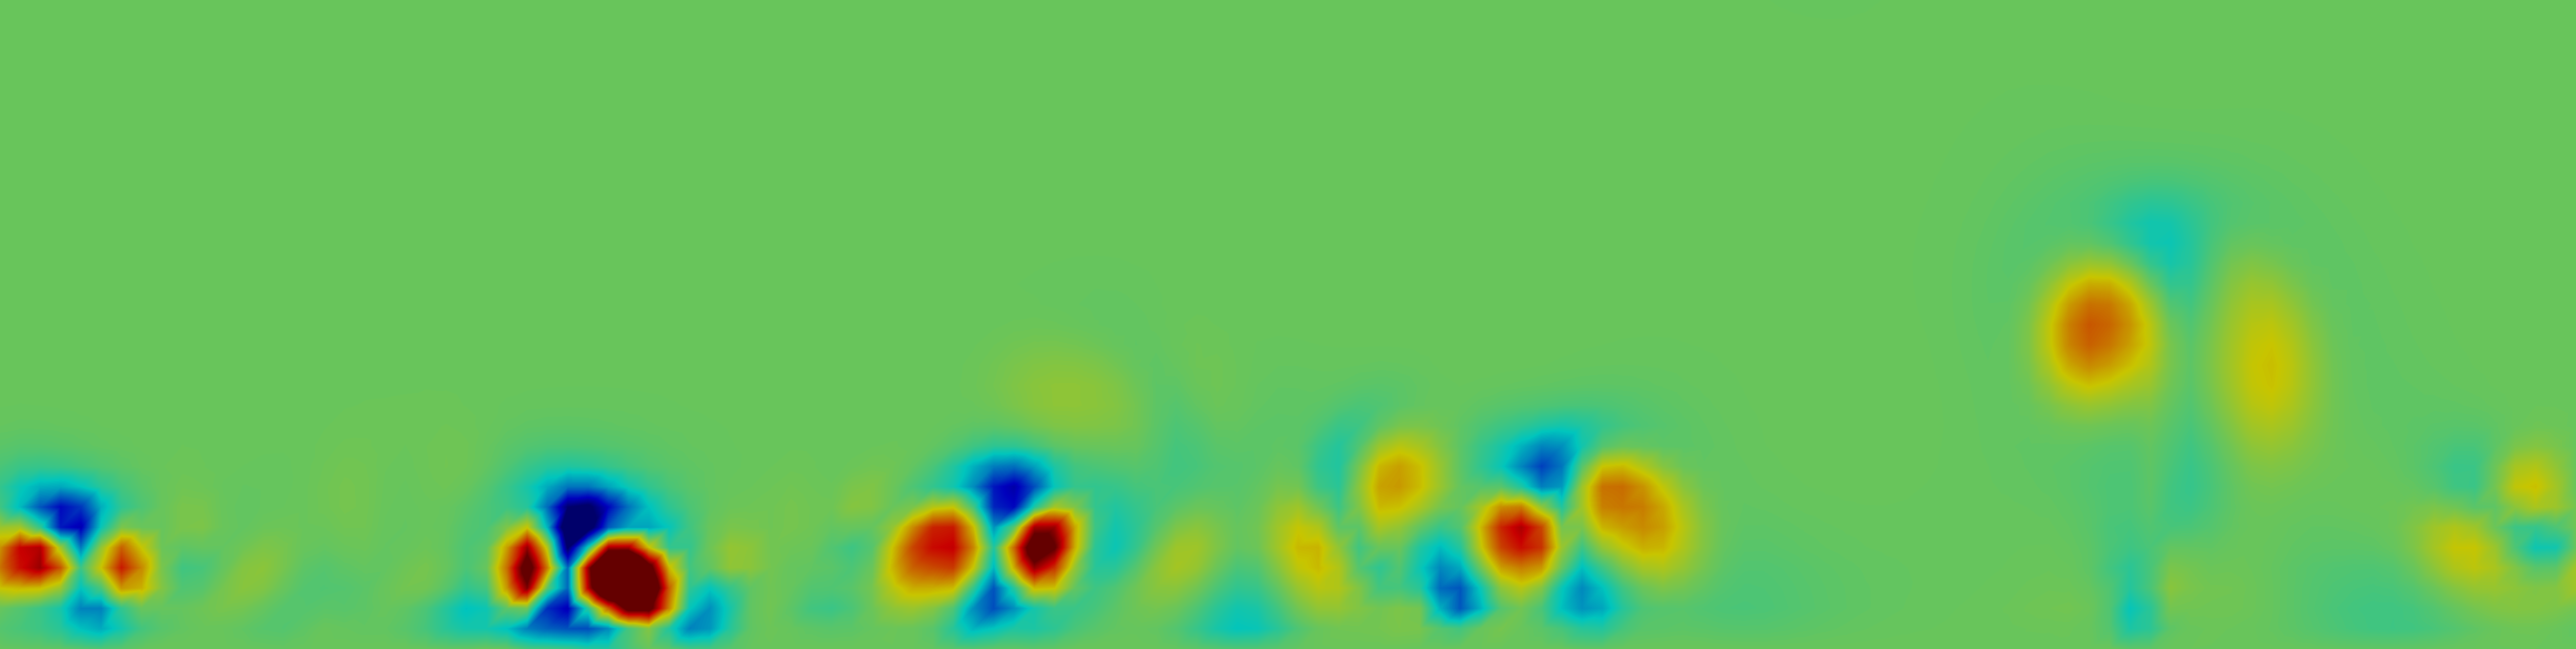
\includegraphics[width=\textwidth]{g0998-q-t8}
          \caption{QuasIncompact3D}
        \end{subfigure}
        \begin{subfigure}[b]{0.99\textwidth}
          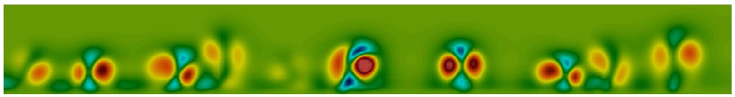
\includegraphics[width=\textwidth]{boussinesq-q-t8}
          \caption{Espath et. al. 2014}
        \end{subfigure}
      \end{figure}
    \end{column}
  \end{columns}
\end{frame}
\begin{frame}
  \frametitle{Example: Q-criterion}
  \framesubtitle{Output}
  
\end{frame}

\begin{frame}
  \frametitle{ToDo}

  \centering

  \begin{itemize}
  \item Parallelisation using \texttt{mpi4py}
  \item Extract data on a plane
  \item Loading every n\textsuperscript{th} node
  \item Handling stretched grids
  \item Filtering of DNS data
  \item Compute spectra
  \item JSON writer - an interactive program to write \texttt{input.json}, similar to
    \texttt{paraview\_incompact3d}
  \end{itemize}
  
  \textbf{Please visit}\\
  \url{github.com/ImperialCollegeLondon/Py4Incompact3D}
\end{frame}

\end{document}


%%%%%%%%%%%%%%%%%%%%%%%%%%%%%%%%%%%%%%%%%%%%%%%%%%%%%%%%%%%%%%%%%%%%%%
%%% py4incompact3d.tex ends here

%%% Local Variables:
%%% mode: latex
%%% TeX-master: t
%%% End:
